\documentclass{article}
\usepackage{graphicx} % Required for inserting images
\usepackage{amsmath}
\usepackage[english, russian] {babel}
\usepackage[utf8]{inputenc}
\usepackage[T2A]{fontenc}
\usepackage{minted}
\usepackage{float}
\usepackage{amssymb}
\usepackage{mathtools}

\title{Компьютерная графика}
\author{Harpie}
\date{February 2025}

\begin{document}

\maketitle

\textbf{17.02.25}

\section{Собъективно-ориентированное программирование}

Это парадигма программирования которая представляет отрезок вменении во время которого возникают определенные события. Программа выполняется не линейно, программа описывается как набор обработчиков/ обработчик события.

Некоторые события происходят автоматически, какие то нужно/можно инициализировать.

Примеры обработчиков:

Paint

Load

Resize

\vspace{5mm}

Некоторые обработчики могут быть инициализированы

Refresh

\section{Полигональная КГ}

Объект описывается с помощью вершин/точек, которые соединенны отрезками. Перед описанием объекта нужно знать и задать координаты точек.

\section{Модели}

Модель строиться набором отрезков, которые определенным образом соединенны в точках, в некоторой системе координат. \textbf{Модельная система координат, объектная система координат,локальная система координат}

Правая система координат - система повернута против часовой стрелки под 90 градусов

Система координат экрана - (нужно заполнить тут) 

Правая декартовая СК (мировая система координат) - "виртуальный мир", в котором существеют модели.

\section{Кадрирование}

Операция кадрирования - совмещенние одного кадра с другим, преобразования одного кадра

Кадр - прямоуглник, стороны которого парарлельны осям координат и у которого есть параметры
 
Размер по горизонтале - Vx

Размер по вертикале - Vy

Координты нижного угла -  Vcx, Vcy


Исходный кадр обозоначается как - Wx, Wy, Wcx, Wcy

Безразмерные координаты :


$x_1 = x-V_cx$ \hspace{21mm} $y_1 = y-V_cy$
\vspace{1mm}

$x_2 = \frac{x-V_cx}{V_x}$ \hspace{22mm} $y_2 = \frac{y-V_cy}{V_y}$
\vspace{1mm}

$x_3 = \frac{x-V_cx}{V_x}*W_x$ \hspace{15mm} $y_3 = \frac{y-V_cy}{V_y}*W_y$
\vspace{1mm}

$x' = \frac{x-V_cx}{V_x}*W_x+W_cx$ \hspace{3mm} $y' = \frac{y-V_cy}{V_y}*W_y+W_cy$

\vspace{5mm}


Если умножить на - 1 еденицу, то картинка перевернется (касается перевернутых картинок)

$x_4=\frac{x-V_cx}{V_x}*W_x+W_cx$ \hspace{3mm}  $y_4= \frac{y-V_cy}{V_y}*W_y-W_cy$

\vspace{1mm}

$x_5 = \frac{x-V_cx}{V_x}*W_x+W_cx$ \hspace{3mm} $y_5 = \frac{y-V_cy}{V_y}*W_x+2W_cy$


$x' = \frac{x-C_cx}{V_x}* W_x+W_cx$ \hspace{3mm}$y' = W_cy- \frac{x-C_cx}{V_x}* W_y$

\vspace{5mm}

\textbf{24.02.25}

\textbf{Продолжение}

$x' = \frac{x-V_{cx}}{V_x} * W_x+W_c$

\vspace{5mm}

$y' = W_y - \frac{y-V_{cy}}{V_y} * W_y$


\section{Преобразование изображения}
\subsection{Элементарные преобразования}

\textbf{1. Перенос/Сдвиг}

Смысл преобразования: объект в одной системе координат 
нужно сдвинуть в "другую систнму координат".

Пример: 

$x_1 \implies x'_1$ между ними расстояние $T_x$ \hspace{5mm} $y_1 \implies y'_1$ между ними расстояние $T_y$

$x_2 \implies x'_2$ между ними расстояние $V_x$ \hspace{5mm} $y_2 \implies y'_2$ между ними расстояние $V_y$


Итог: $x'=x+T_x$ \hspace{5mm} $y'=y+T_y$

\vspace{5mm}

\textbf{2. Масштабирвоание относительно начала координат}

Это озночает, все точки преобразуются за исключением начальной точки.
На месте остается только точка начала координат.

Пример:

$3 \implies 4.5$ и т.д

Итог: $x'=x*S_x$ \hspace{5mm} $y'=y*S_y$ 

\vspace{5mm}

\textbf{3. Поворот относительно начала координат против часовой стрелки на угол $\vartheta$}

Нужно соеденить лучом точку с началом координат. Преоброзовать точку означает, повернуть этот
отрезок на заданный угол $\vartheta$. В результате полчвется новая точка.

$x' = r cos(\alpha + \vartheta)^x = r cos \alpha cos \vartheta - r sin \alpha sin \varTheta
= x cos \vartheta - y sin \vartheta$

$y' = r sin(\alpha + \vartheta)^x = r sin \alpha cos \vartheta + r sin \vartheta cos \alpha
= y cos \vartheta + x sin \vartheta$

Итог : $x' = x cos \vartheta - y sin \vartheta$ \hspace{5mm}$y'= y cos \vartheta + x sin \vartheta$

\textbf{4. Зеракальное отражение. Частный случай масштабирвоание}

$x' = x*-1$ \hspace{5mm} $y' = y*-1$




\section{Совмещенние преобразований}

Пример: поворот на угол $\vartheta$ против часовой стрелки относительно т. $A(x_a, y_a)$

$x^{(1)}=x-x_a$ \hspace{5mm} $y^{(1)}=y-y_a$ 

$x^{(2)}=x^{(1)} cos \vartheta - y^{(2)} sin \vartheta $ \hspace{5mm}
$y^{(2)}=x^{(1)} csin \vartheta + y^{(2)} cos \vartheta $

\vspace{2mm}

$x' = x^{(2)}+x_a = (x-x_a) cos \vartheta - (y-y_a) sin \vartheta +x_a$

$y' = y^{(2)}+y_a = (x-x_a) csin \vartheta + (y-y_a) cos \vartheta +y_a$


\vspace{5mm}

$\begin{bmatrix}
    x' \\
    y' \\ 
\end{bmatrix}
=
\begin{bmatrix}
    a_{11} & a_{12}  \\[0.3em]
    a_{21} & a_{22}  \\[0.3em]
\end{bmatrix}
\begin{bmatrix}
    x \\
    y \\
\end{bmatrix}$

\subsection{Однородные координаты}
    \subsubsection{Евклидовые координаты}

    В однородных координатах координаты объекта задается с точностью какого то множетеля. Например,
    для прямой вида $A_x + B_y + C = 0$. Можно скзаать, что координаты прямой задаются тройкой $(A,B,C)$.
    В таком случае, если домножить эту тройку, то она все еще будет указывать на иходную прямую.

    Для евклидовой точки $(x,y)$ выберем некоторую произвольную


    \textbf{ Переход от однородных в евклидовые координаты}

    Предположим были однородные координаты $(\chi, \gamma, \alpha)$ 
    и нам нужно получить $(\chi ', \gamma ', \alpha ')$

    \subsection{Однородные преобразоавания}

    Формула для масштабирвоание 

    $\chi ' = \chi S_\chi$

    $\gamma ' = \gamma S_\gamma$

    $\alpha ' = \alpha$

    Матрица масштабирвоания 

    $\begin{bmatrix}
        \chi' \\
        \gamma ' \\ 
        \alpha ' \\

    \end{bmatrix}
    =
    \begin{bmatrix}
        S_x & 0  & 0 \\[0.3em]
        0 & S_y  & 0 \\[0.3em]
        0 & 0  & 1 \\[0.3em]
    \end{bmatrix}
    \begin{bmatrix}
        \chi \\
        \gamma  \\ 
        \alpha  \\
    \end{bmatrix}$


    Матрица поворота


    $\begin{bmatrix}
        \chi' \\
        \gamma ' \\ 
        \alpha ' \\

    \end{bmatrix}
    =
    \begin{bmatrix}
        cos \vartheta & -sin \vartheta  & 0 \\[0.3em]
        sin \vartheta &  cos \vartheta  & 0 \\[0.3em]
        0 & 0  & 1 \\[0.3em]
    \end{bmatrix}
    \begin{bmatrix}
        \chi \\
        \gamma  \\ 
        \alpha  \\
    \end{bmatrix}$
\hspace{5mm}

$\chi ' = \alpha x' = \alpha x + Y_x \alpha$

$\gamma ' = \gamma x' = \gamma x + Y_x \alpha$

$\alpha ' = \alpha$


Матрица для переноса

$\begin{bmatrix}
    \chi' \\
    \gamma ' \\ 
    \alpha ' \\

\end{bmatrix}
=
\begin{bmatrix}
    1 & 0  & T_x \\[0.3em]
    0 & 1  & T_y \\[0.3em]
    0 & 0  & 1 \\[0.3em]
\end{bmatrix}
\begin{bmatrix}
    \chi \\
    \gamma  \\ 
    \alpha  \\
\end{bmatrix}$

Универсальная формула

$\begin{bmatrix}
    \chi' \\
    \gamma ' \\ 
    \alpha ' \\

\end{bmatrix}
=
\begin{bmatrix}
    cos \vartheta & -sin \vartheta  & 0 \\[0.3em]
    sin \vartheta &  cos \vartheta  & 0 \\[0.3em]
    0 & 0  & 1 \\[0.3em]
\end{bmatrix}
\begin{bmatrix}
    S_x & 0  & 0 \\[0.3em]
    0 & S_y  & 0 \\[0.3em]
    0 & 0  & 1 \\[0.3em]
\end{bmatrix}
\begin{bmatrix}
    1 & 0  & T_x \\[0.3em]
    0 & 1  & T_y \\[0.3em]
    0 & 0  & 1 \\[0.3em]
\end{bmatrix}
\begin{bmatrix}
    \chi \\
    \gamma  \\ 
    \alpha  \\
\end{bmatrix}$


\textbf{03.03.25}


$P'= MP$ В таком виде записывается матричное преообразование

P - столбец

M - матрица

P=
$\begin{bmatrix}
    \chi \\
    \gamma  \\ 
    \alpha  \\

\end{bmatrix}$
P=
$\begin{bmatrix}
    \chi' \\
    \gamma ' \\ 
    \alpha ' \\

\end{bmatrix}$


M' - обратная матрица


$P=M'(MP) \\Rightarrow  M'=M^-1$


\subsection{Преобразование перенос}


Translate ($T_x, T_y$) = 
$\begin{bmatrix}
    1 & 0  & T_x \\[0.3em]
    0 & 1  & T_y \\[0.3em]
    0 & 0  & 1 \\[0.3em]
\end{bmatrix}
\begin{bmatrix}
    1 & 0  & -T_x \\[0.3em]
    0 & 1  & -T_y \\[0.3em]
    0 & 0  & 1 \\[0.3em]
\end{bmatrix}$


T($T_x,T_y$)


\subsection{Преобразование масштабирвоание}

Scale ($S_x,S_y$) 
$\begin{bmatrix}
    S_x & 0  & 0 \\[0.3em]
    0 & S_y  & 0 \\[0.3em]
    0 & 0  & 1 \\[0.3em]
\end{bmatrix}
\begin{bmatrix}
    1/S_x & 0  & 0 \\[0.3em]
    0 & 1/S_y  & 0 \\[0.3em]
    0 & 0  & 1 \\[0.3em]
\end{bmatrix}$

S($S_x,S_y$) 

\subsection{Преобразование поворот}

Rotate($\vartheta$) = 
$\begin{bmatrix}
    cos \vartheta & -sin \vartheta  & 0 \\[0.3em]
    sin \vartheta &  cos \vartheta  & 0 \\[0.3em]
    0 & 0  & 1 \\[0.3em]
\end{bmatrix}
\begin{bmatrix}
    cos \vartheta & sin \vartheta  & 0 \\[0.3em]
    -sin \vartheta &  cos \vartheta  & 0 \\[0.3em]
    0 & 0  & 1 \\[0.3em]
\end{bmatrix}$


\section{Совмещенное преобразование}

Смысл:

$P' = (M_2...M_3,M_2,M_1)P$

$E = M' (M_3,M_2,M_1)$

$M' = M' (M_{\Delta }^{-1}, M_{2}^{-1},M_{3}^{-1})$


\section{Принцип двойтсвенности}
Двойственное преобразование

У нас есть матрица

$\begin{bmatrix}
    1 & 0 & T_x \\
    0 & 1 & T_y \\
    0 & 0 & 1 \\
\end{bmatrix}$

Масштабирвоание равно преобразованию....


Напоминание: Операция кордирования $x' = \frac{x-V_{cx}}{V_x} W_x + W_{cx}$

$y' = \frac{y-V_{cy}}{V_y} W_y + W_{cy}$

$\frac{W_x}{V_x} < \frac{W_y}{V_y}$


$\frac{2}{V_x} < \frac{2}{V_y}$


$1 = \frac{2}{2} < \frac{V_x}{V_y}$ - aspect - соотношение сторон

Если соотношение сторон больше 1 масштабируем по x, если же наоборот то по y.
 (Для вписания картинки в квадрат )

$\frac{W_x}{V_x}$ или $\frac{W_y}{V_y}$


$\frac{2}{V_x}$ или $\frac{2}{V_y}$




$ \begin{cases}
 V_{x}^{'} \\  
\hspace{1cm} \text{Размеры модели после вписания в квадрат 2x2} \\
V_{y}^{'} \\
\end{cases} $


\begin{figure} [H]
    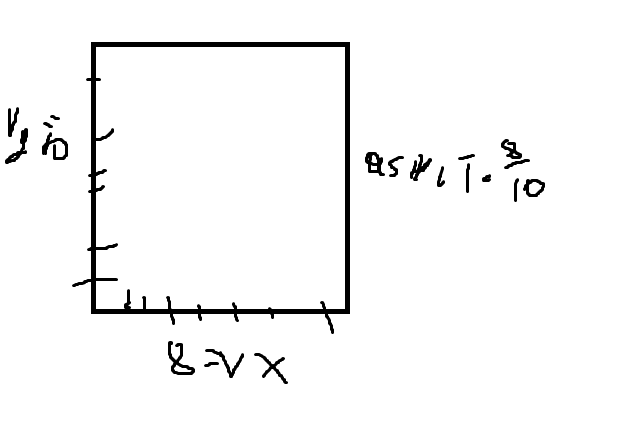
\includegraphics[width=0.50\linewidth]{1.png}
\end{figure}

\begin{figure} [H]
    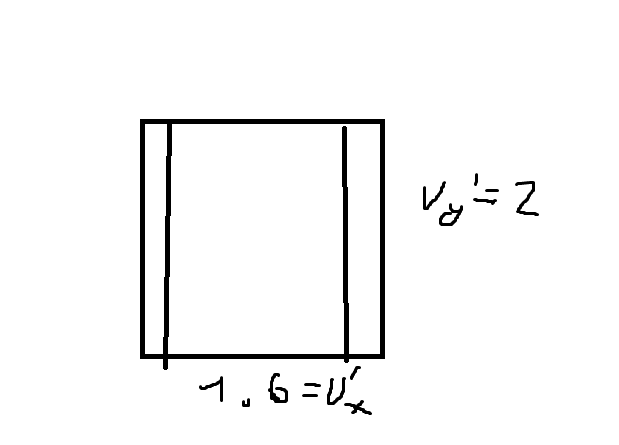
\includegraphics[width=0.50\linewidth]{2.png}
\end{figure}

\textbf{Команды:}

translate x  y


rotate $\vartheta$


scale S


figure 

Вспомогательные команды

popTransform - забираем из стка


pushTransform - добавляем в стек

\vspace{1cm}

scale 1.25

pushTransform

translate 0 -R

translate x y



translate -x -y

rotate 22.5

translate x y
\begin{figure} [H]
    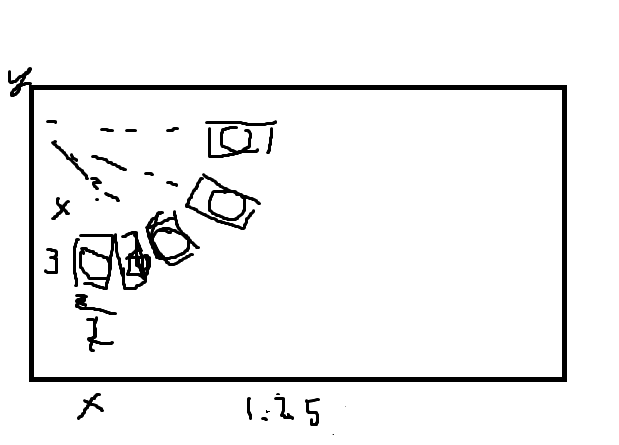
\includegraphics[width=0.50\linewidth]{3.png}
\end{figure}




Сокращение картинки:

scale 1.25

translate 0 -R

pushTransform

translate x y

figure

popTransform

rotate 22.5

pushTransform

translate x Y

figure


$\begin{cases}
    
pushTransform \\

rotate 22.5 \\

pushTransform \\

translate x y \\

figure \\

\end{cases}$

popTransform



\textbf{10.03.25}

\section{Операции над векторами}
\subsection{Двумерные вектора}
У веторов две характиристики:

длина

+

направлнение

Подобные вектора называется свободными векторами
если, есть точка из которой он начинается, 
то он называется связанным

Угол вектора $(r,\varphi)$

Угол ветора против часовой стрелки

\begin{figure} [H]
    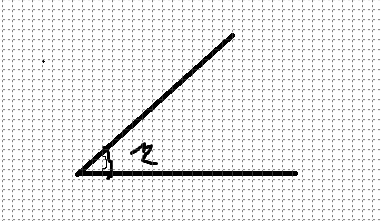
\includegraphics[width=0.50\linewidth]{Снимок экрана 2025-03-10 121857.png}
\end{figure}




\begin{figure} [H]
    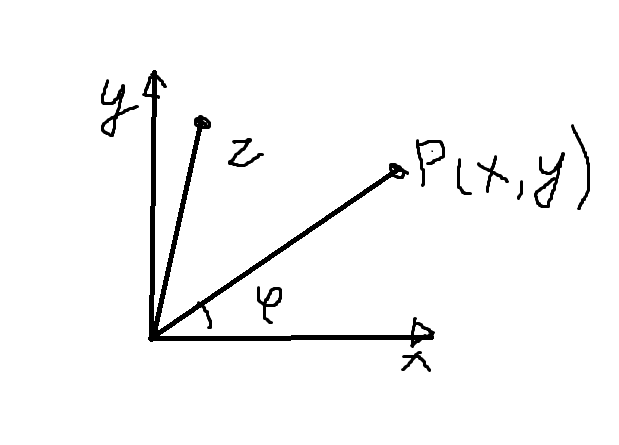
\includegraphics[width=0.50\linewidth]{4.png}
\end{figure}
Радиус вектор точка P

$\bar{P} (x,\varphi)$

$x = r cos \varphi$

$y = r sin \varphi$




\begin{figure} [H]
    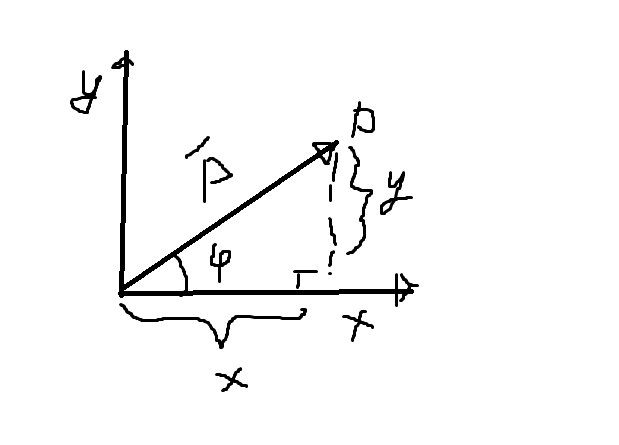
\includegraphics[width=0.50\linewidth]{5.png}
\end{figure}


\textbf{Сложение векторов(сумма)}

$\bar{u} u \bar{v}$

$\bar{u} + \bar{v}$


$\bar{u} = (u_x,u_y)$

$\bar{v} = (v_x,v_y)$

$\bar{u} + \bar{v} = (u_x+v_x,u_y+v_y)$


\begin{figure} [H]
    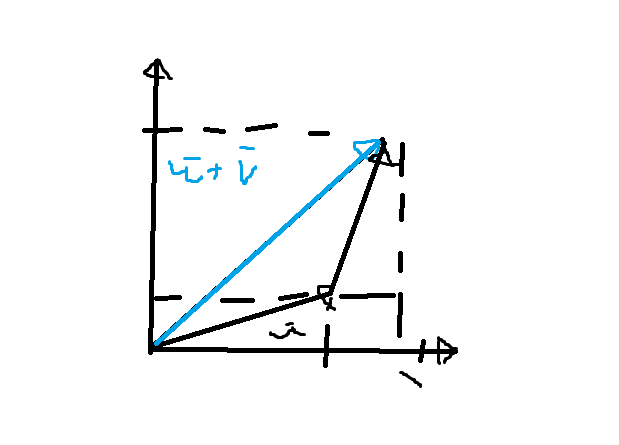
\includegraphics[width=0.50\linewidth]{6.png}
\end{figure}

\textbf{Разность векторов}
$\bar{u} u \bar{v}$

$\bar{u} - \bar{v}$


$\bar{u} - \bar{v} = (u_x-v_x,u_y-v_y)$

\begin{figure} [H]
    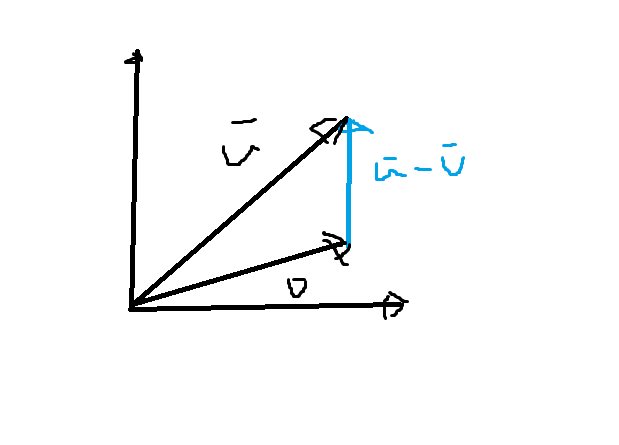
\includegraphics[width=0.50\linewidth]{7.png}
\end{figure}


\textbf{пупуп }


\begin{figure} [H]
    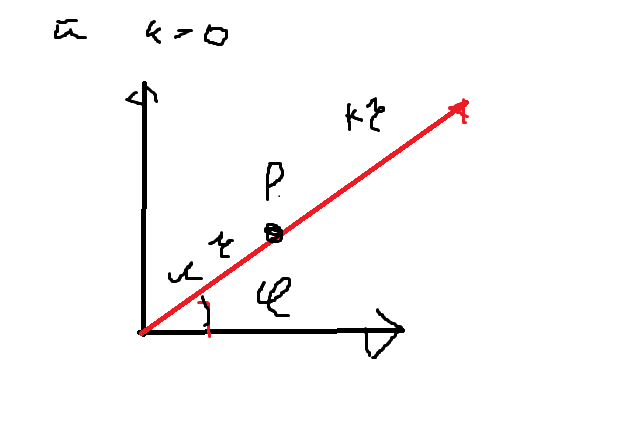
\includegraphics[width=0.50\linewidth]{8.png}
\end{figure}

$k\bar{u} = (ku_x,ku_y)$


\textbf{Скалярное произведение векторов}

$\bar{u}  \bar{v}$

$\bar{u} * \bar{v} = |\bar{u}| |\bar{v}| cos \widehat{\bar{u} \bar{v}} $

$\bar{u} = (r,\varphi)$

$|\bar{u}| = r$

$\bar{u} = \bar{u_x+\bar{u_y}}$

$\bar{u} * \bar{v} = (\bar{u_x+\bar{u_y}})*(\bar{v_x} + \bar{v_y})= $
$(|u_x|e_1 + |u_y|e_2) *(|v_x|e_1 *|v_x|e_1)$


$\bar{u}*\bar{v} = |\bar{u_x}||\bar{v_x}||\bar{u_x}+|\bar{v_y}| $ - основная формула
\begin{figure} [H]
    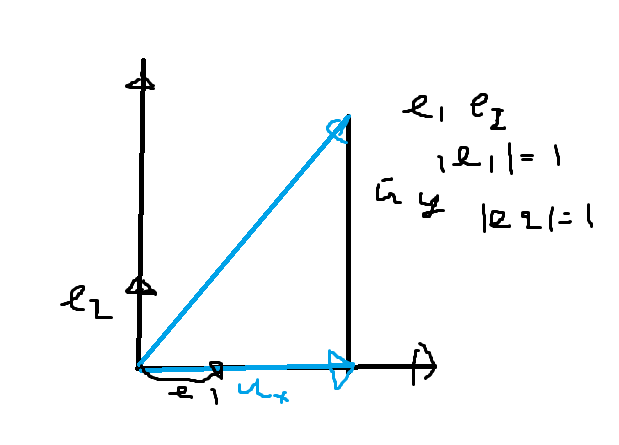
\includegraphics[width=0.50\linewidth]{9.png}
\end{figure}


$\bar{u} \bar{i}$

$\bar{u}*\bar{i} = |\bar{u}| |\bar{i}| cos \widehat{\bar{u} \bar{i}} =$
$|\bar{u}| cos\widehat{\bar{u} \bar{i}}$




\begin{figure} [H]
    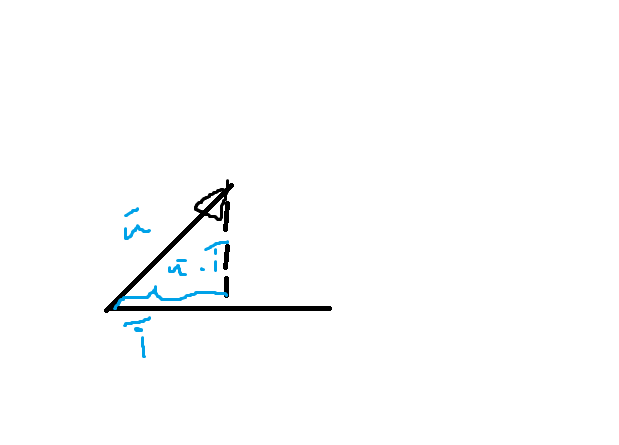
\includegraphics[width=0.50\linewidth]{10.png}
\end{figure}


dot-prodect - Скалярное произведение

\textbf{Псевдоскалярное произведение}

$\bar{u} \bar{v}$

$\bar{u} x \bar{v} = |\bar{u}|\bar{v}|sin < \bar{u} \bar{v}$

$\bar{u} x \bar{v} = -\bar{u} x \bar{v}$


$ e_1 x e_1 = 0
e_1 x e_2 = 1
e_2 x e_1 = -1
e_2 x e_2 = 0
= u_xv_y - u_yv_x > \bar{u} x \bar{v} = $ 
$ \begin{bmatrix}
    u_x & u_y \\
    v_x & v_y \\

\end{bmatrix} $

cross-prodect - Псевдоскалярное произведение 



\subsection{Трехмерные вектора}


\begin{figure} [H]
    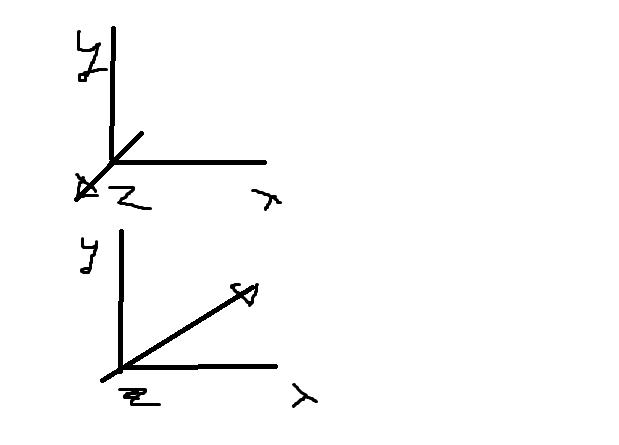
\includegraphics[width=0.50\linewidth]{КоординатыПравЛев.png}
    \text{Левосторонняя и правостороняя}
\end{figure}


\begin{figure} [H]
    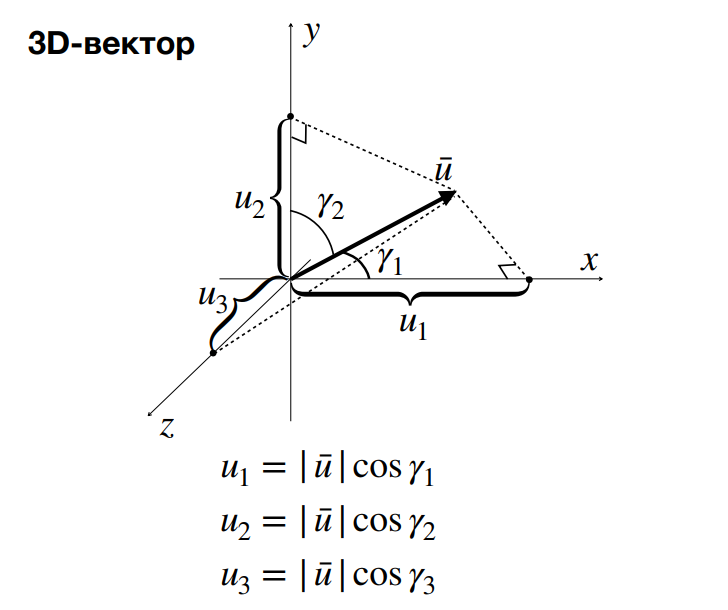
\includegraphics[width=0.50\linewidth]{Снимок экрана 2025-03-10 131058.png}
\end{figure}

\begin{figure} [H]
    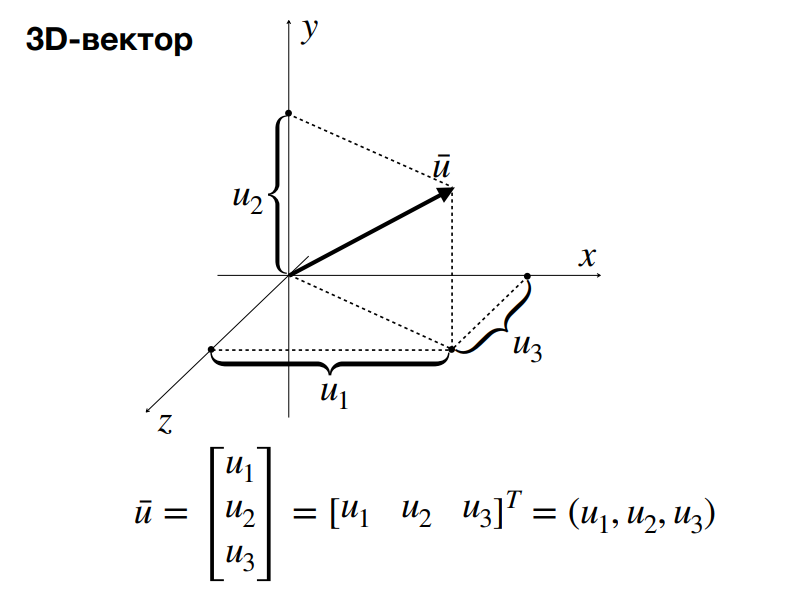
\includegraphics[width=0.50\linewidth]{Снимок экрана 2025-03-10 131148.png}
\end{figure}


\begin{figure} [H]
    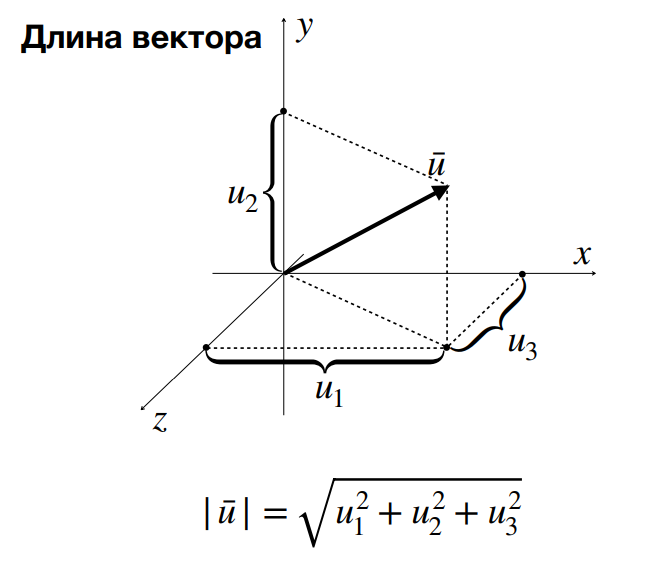
\includegraphics[width=0.50\linewidth]{Снимок экрана 2025-03-10 131219.png}
\end{figure}

\begin{figure} [H]
    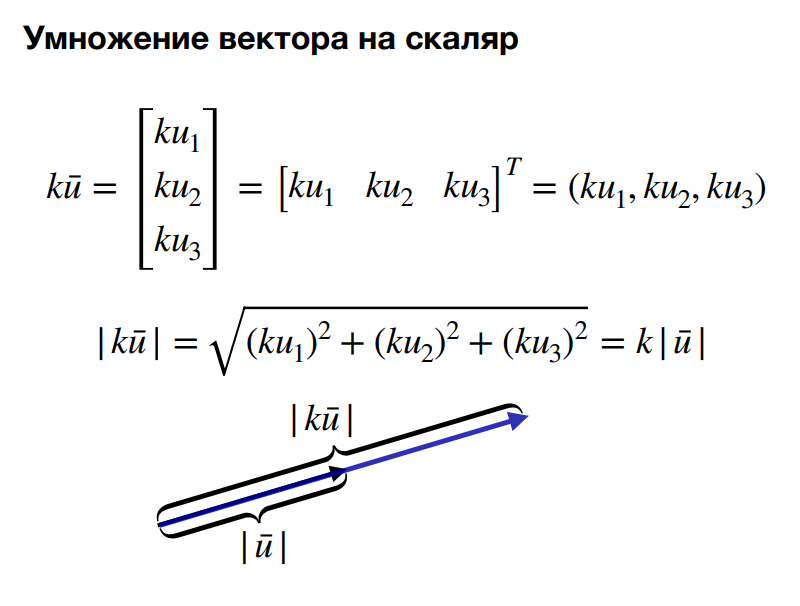
\includegraphics[width=0.50\linewidth]{Снимок экрана 2025-03-10 131255.png}
\end{figure}


\begin{figure} [H]
    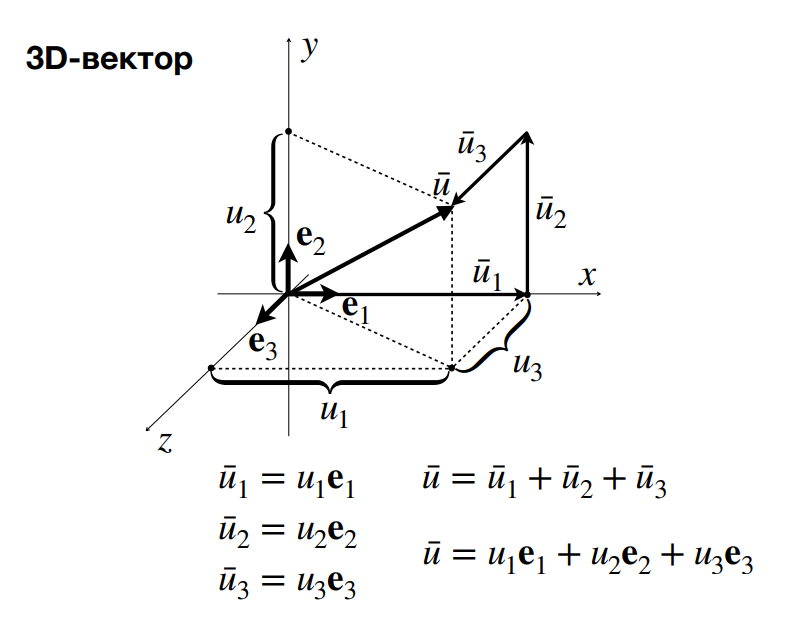
\includegraphics[width=0.50\linewidth]{Снимок экрана 2025-03-10 131408.png}
    \text{Сложение вектора по координатам}
\end{figure}


\textbf{!Скалярное произведение аналогично двухмерному}


\begin{figure} [H]
    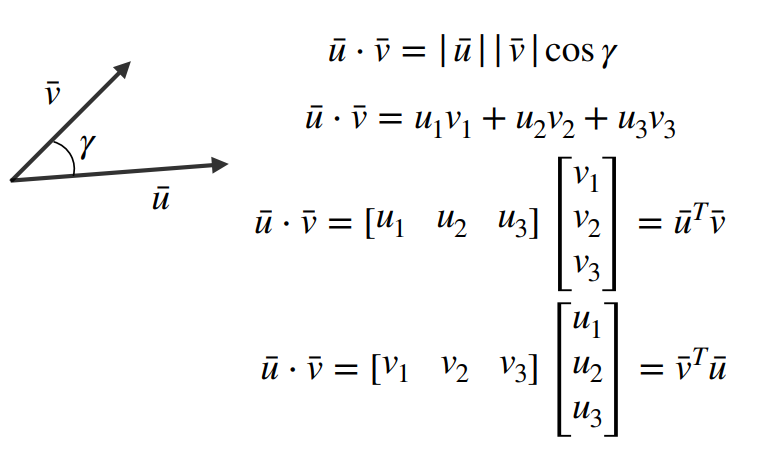
\includegraphics[width=0.50\linewidth]{Снимок экрана 2025-03-10 131719.png}
    \text{Через матрицу}
\end{figure}

\textbf{Векторное произведение}
\begin{figure} [H]
    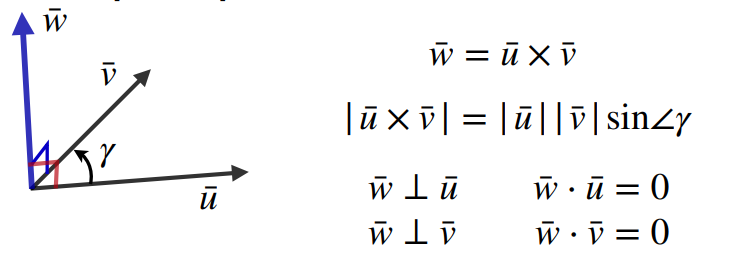
\includegraphics[width=0.50\linewidth]{Снимок экрана 2025-03-10 131820.png}
\end{figure}


Угол может быть как положительным, так и отрицательным

Не важно в какую сторону отмереяться угол

Если положительный результат, то вверх, 
отрицательный же вниз

\begin{figure} [H]
    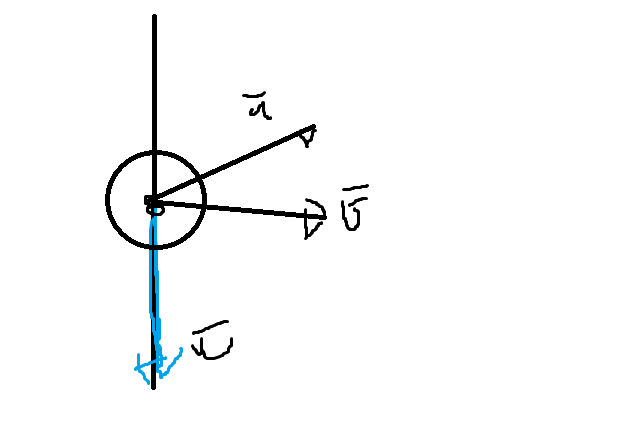
\includegraphics[width=0.50\linewidth]{11.png}
\end{figure}




\begin{figure} [H]
    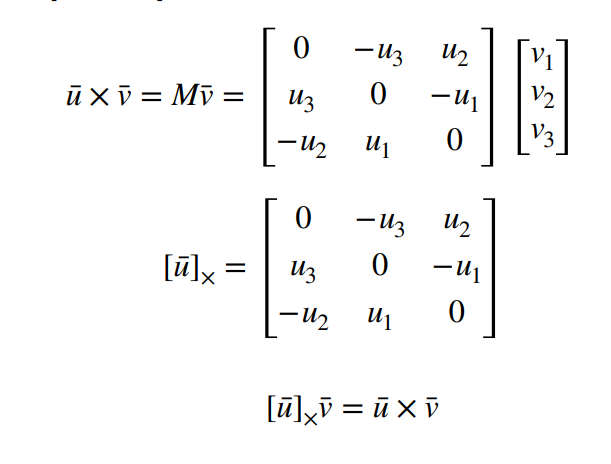
\includegraphics[width=0.50\linewidth]{Снимок экрана 2025-03-10 133749.png}
    \text{Матрица векторного произведения}
\end{figure}



\textbf{17.03.25}


\section{Одномерноые координаты}

$e = (A,B,C) (0,0,3)$

$A_x+B_y+C=0$

$P ~ (\chi,\gamma, \alpha) = (\frac{\chi}{\alpha}, \frac{\gamma}{\alpha})$

$(2,3,0)$

\vspace{3mm}

$A_\chi + B_\gamma + C+\alpha = 0$

$(A,B,C) (\chi,\gamma,\alpha) = 0$

$P_1(\chi_1,\gamma_1,\alpha_1)$ и $P_2(\chi_2,\gamma_2,\alpha_2) $

\vspace{3mm}

$P_1 x P_2 = e$

$e_1 x e_2 = P$

\textbf{Одномерноые координаты не будут использоваться в этом курсе, но пусть будут как факт}


Плюкерова координата - $\beta=LP$

L - представление как матрицы 4x4

\textbf{Все выше перечисленное не бует на экзамене, это чисто для общего развитися}

\section{Построение 2D - графика}

Задана некая функция, нужно изобразить на экране.
Функция бесконечная, как и графика.
Нужно определить кадр, выделить его.
Здаем кадр на экране.


\begin{figure} [H]
    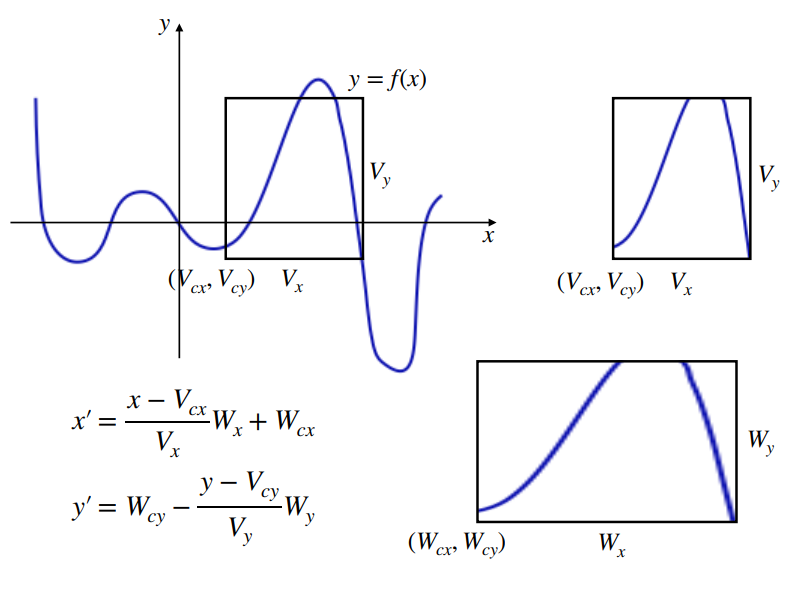
\includegraphics[width=0.70\linewidth]{Снимок экрана 2025-03-17 123016.png}
\end{figure}


\begin{figure} [H]
    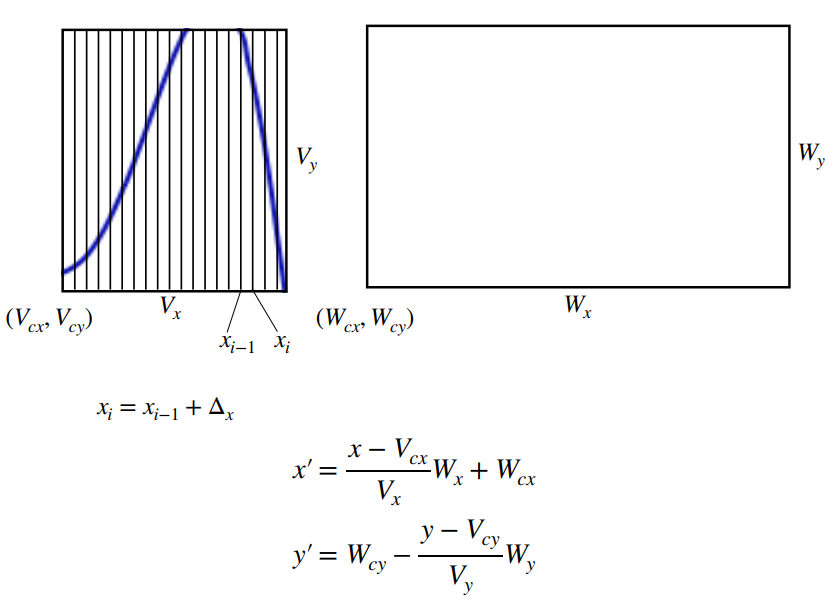
\includegraphics[width=0.70\linewidth]{Снимок экрана 2025-03-17 123224.png}
\end{figure}

$\Delta$ - шаг 

Что получается

$x_0 = V_{cx}\longrightarrow x_{0}^{'} = W_{cx}$ - кадрирование

$y_0 = f(x_0)\longrightarrow y_{0}^{'}$ - кадрирование

$x_i = x_{i-1} + x \longrightarrow x_{0}^{'}$ - кадрирование


$y_i = f(x_0) + x \longrightarrow y_{0}^{'}$ - кадрирование

отрезок от $x_{i-1}^{'}, y_{i-1}^{'}$ до $x_{i}^{'}, y_{i}^{'}$

цикл $x_i < W_{cx}+W_x$

\vspace{3mm}

Как выбрать $\Delta_x$?

Нужно отталкиваться от экрана, в завимисмоти от этого и выбиратьеся $\Delta_x$.
Экран растровое пространство. По сути это сетка - точка растра.

\begin{figure} [H]
    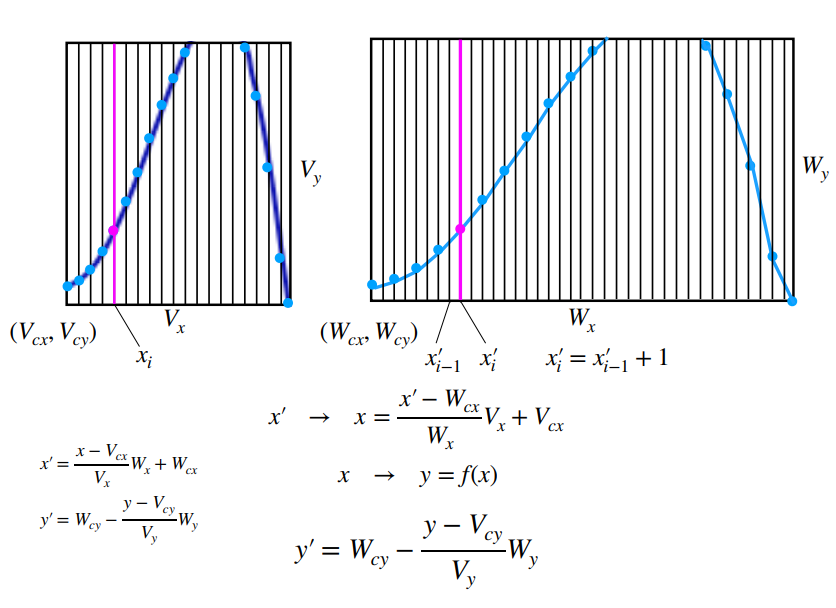
\includegraphics[width=0.70\linewidth]{Снимок экрана 2025-03-17 125154.png}
\end{figure}


Цикл отриосовки:

пока $x_{i}^{'} <= W_{cx}+W_x$

$x_{i}^{'} = x_{i-1}^{'}+1 \longrightarrow x_i$ кадр

$y_{i}^{'} \longleftarrow y_i (f_i)$ кадр

обработка от $(x_{i-1}^{'}, y_{i-1}^{'})$ до $(x_{i}^{'}, y_{i}^{'})$

$x_i = x_{i-1} + \frac{V_x}{W_x}$

\vspace{3mm}

Все усложняется, когда появляется разрыв... 
\begin{figure} [H]
    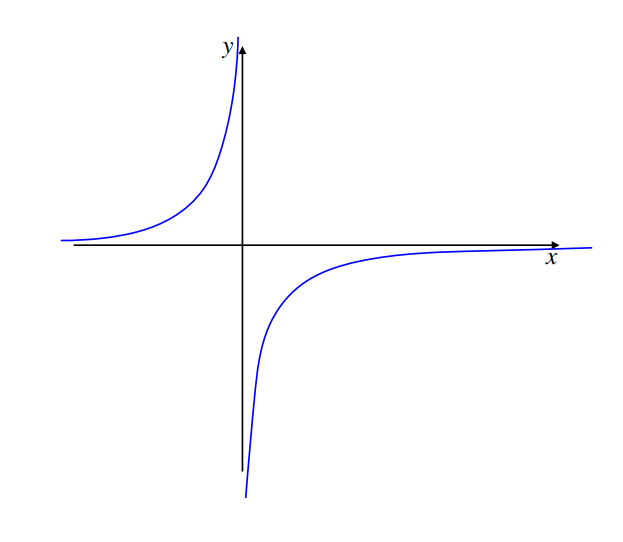
\includegraphics[width=0.70\linewidth]{Снимок экрана 2025-03-17 130158.png}
\end{figure}

\begin{figure} [H]
    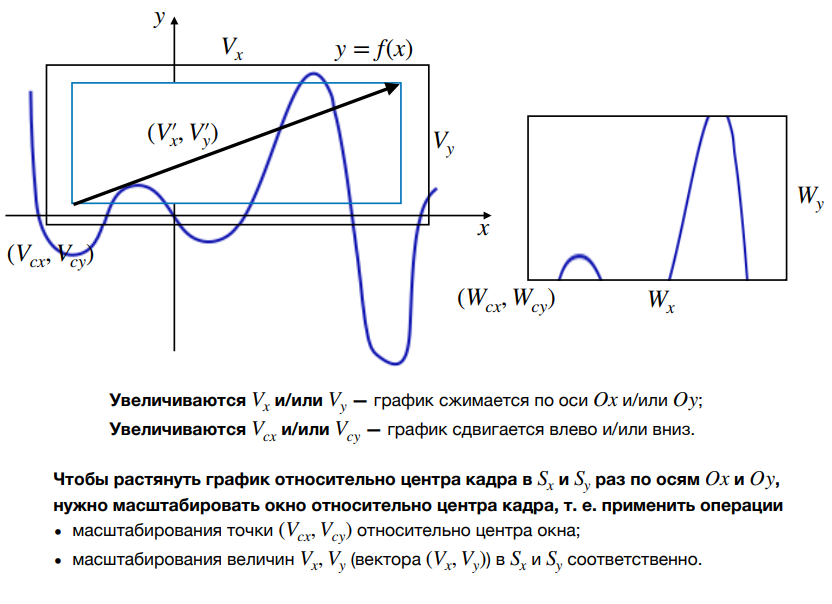
\includegraphics[width=0.70\linewidth]{Снимок экрана 2025-03-17 131649.png}
\end{figure}



\begin{figure} [H]
    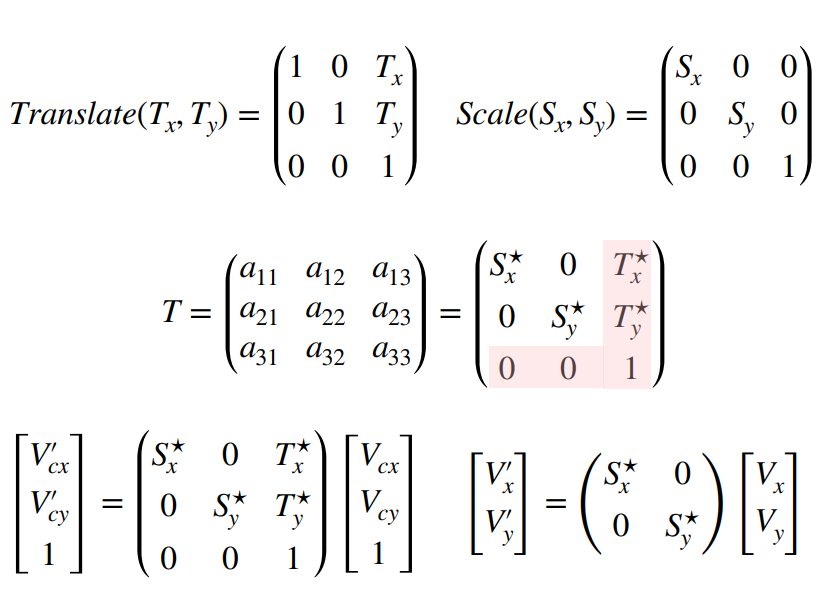
\includegraphics[width=0.70\linewidth]{Снимок экрана 2025-03-17 132004.png}
\end{figure}

Так будет масштобироваться в окне

\section{Построение 3D-граифка}

Трехмерный график формирктся из двумерных графиков


Пусть:


Бужем обозначать $y = f(x,z)$. Теперь график зависит еще и от z

\begin{figure} [H]
    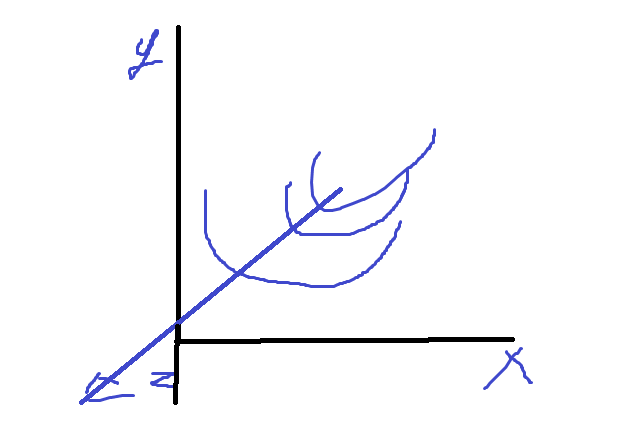
\includegraphics[width=1\linewidth]{tri.png}
\end{figure}


\begin{figure} [H]
    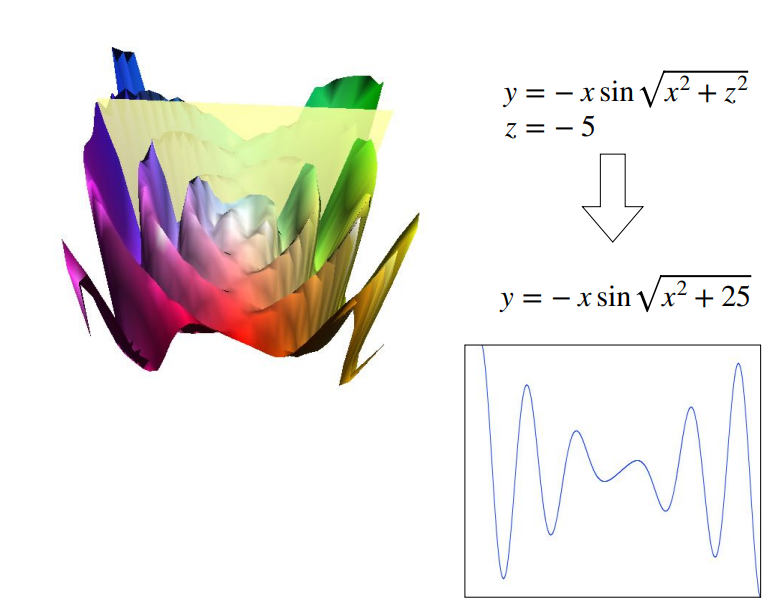
\includegraphics[width=1\linewidth]{Снимок экрана 2025-03-17 132538.png}
\end{figure}


Для рисования такого используется "Алгоритм художника".
Вначале начинаем с заднегго плана и от него идет вплоть до самого ближнего плана


\begin{figure} [H]
    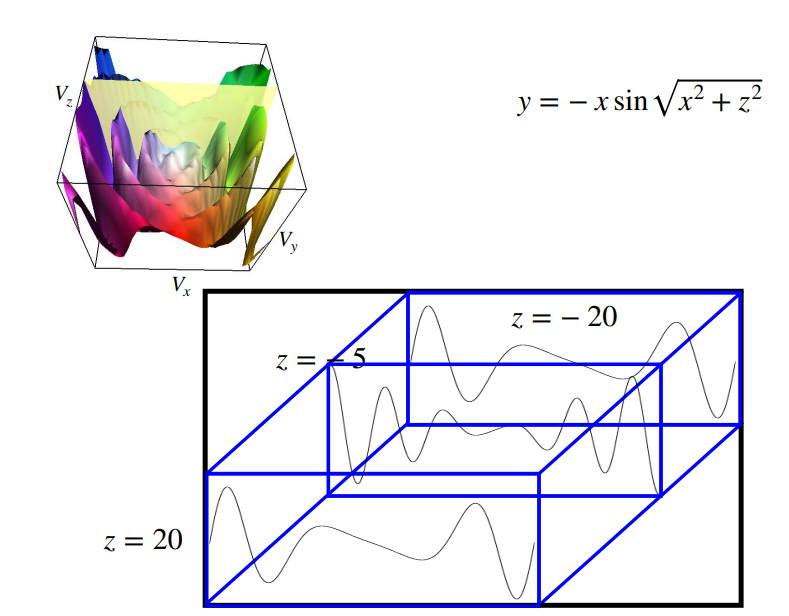
\includegraphics[width=1\linewidth]{Снимок экрана 2025-03-17 132808.png}
\end{figure}



\textbf{24.03.25}

Пропуск лекции из-за досдачи

\textbf{31.03.25}

\subsection{3D - преобразоавания}

\begin{figure} [H]
    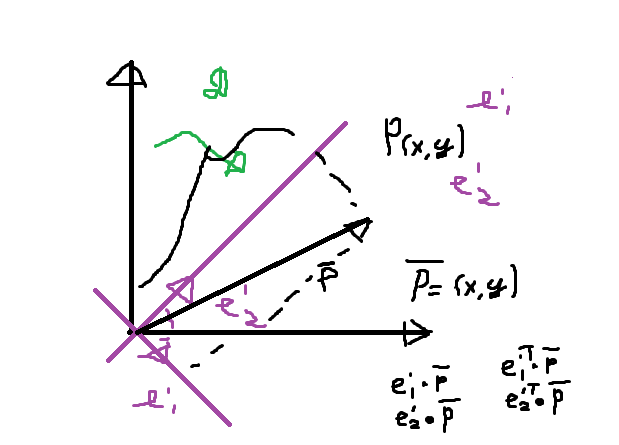
\includegraphics[width=0.70\linewidth]{тра.png}
\end{figure}

Матричная форма $\bar{p'}=$
$\begin{bmatrix}
    e^{'T}_{1} \\
    e^{'T}_{2} \\
\end{bmatrix}
\bar{p}
$

\begin{figure} [H]
    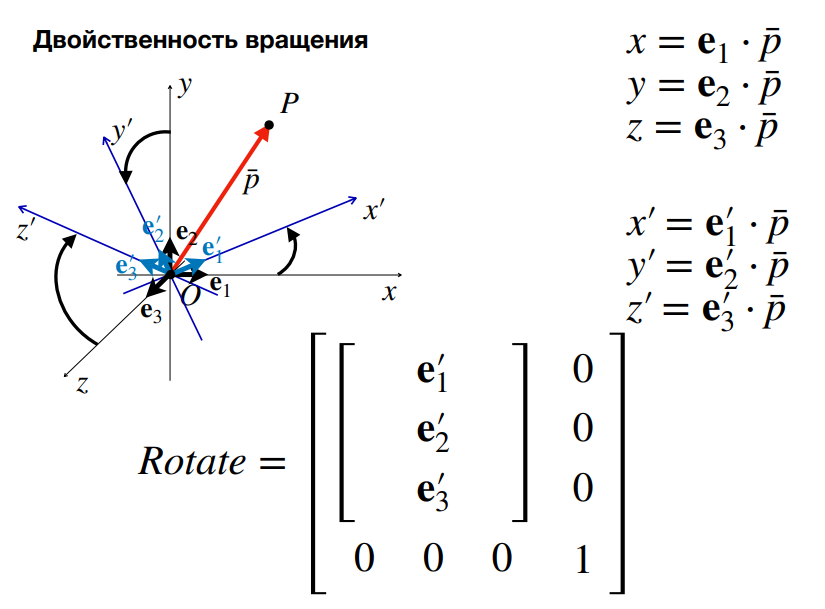
\includegraphics[width=0.70\linewidth]{Снимок экрана 2025-03-31 123501.png}
\end{figure}


\section{Система координат наблюдателя}

\textbf{Замечание}

Модель это набор отрезков, на данный момент.

Вершины заданы в какой-то система координат.

Преобразование накапливается.

Для каждого набора точек, своя модель преобразоавания.

Есть неизменяемые вершинные данные, изменяются только преобразования.


\begin{figure} [H]
    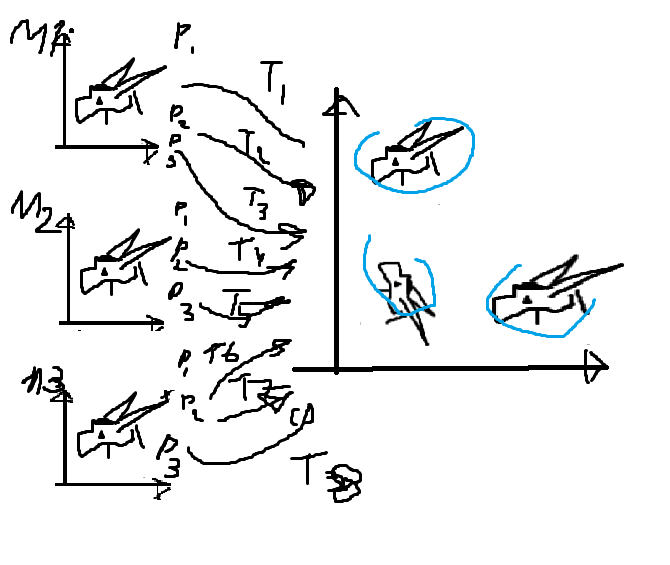
\includegraphics[width=0.70\linewidth]{пре.png}
\end{figure}

\vspace{1cm}

Точка наблюдене - точка зрения наблюдателя(camera). 

Вектор наблюдения - вектор направленый от взляда наблюдателя в точку наблюдения.

Система координат - правая декартовая система координат, лежащая от глаз наблюдателя

Ось x направленна влевео вниз от наблюдателя

Ось y направленна вверх от наблюдателя

Ось z направленна вправо от наблюдателя

\begin{figure} [H]
    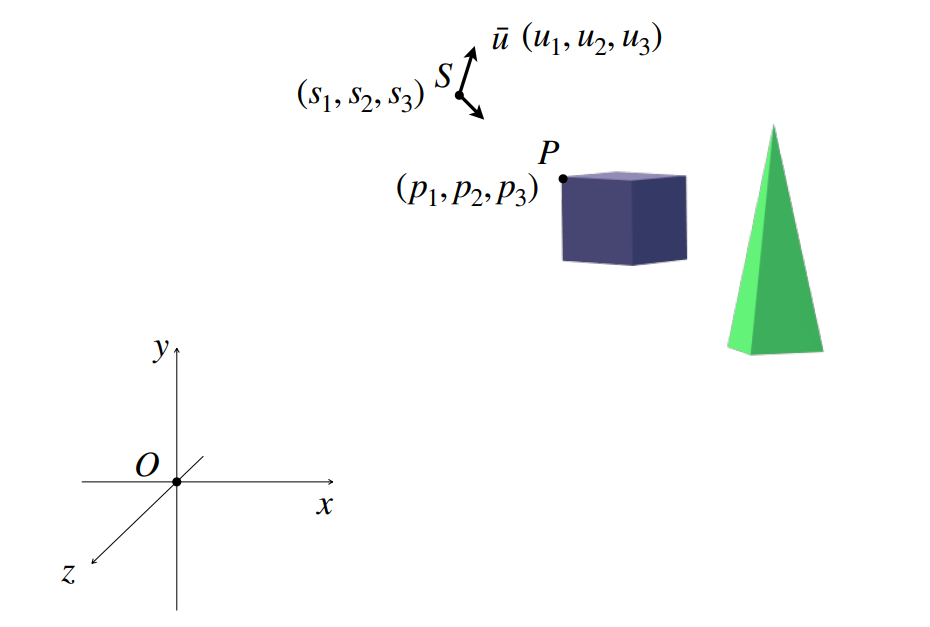
\includegraphics[width=0.70\linewidth]{Снимок экрана 2025-03-31 125809.png}
\end{figure}

\vspace{5mm}

\textbf{Преобразование:}

\vspace{2mm}
1. Поворот

$\begin{bmatrix}
    0 && 0 && 0 && -S_1 \\
    0 && 1 && 0 && -S_2 \\
    0 && 0 && 1 && -S_3 \\
    0 && 0 && 0 && 1 \\
\end{bmatrix}
$

\vspace{5mm}

2. Вращение. Нужно определить матрицу вращения

\begin{figure} [H]
    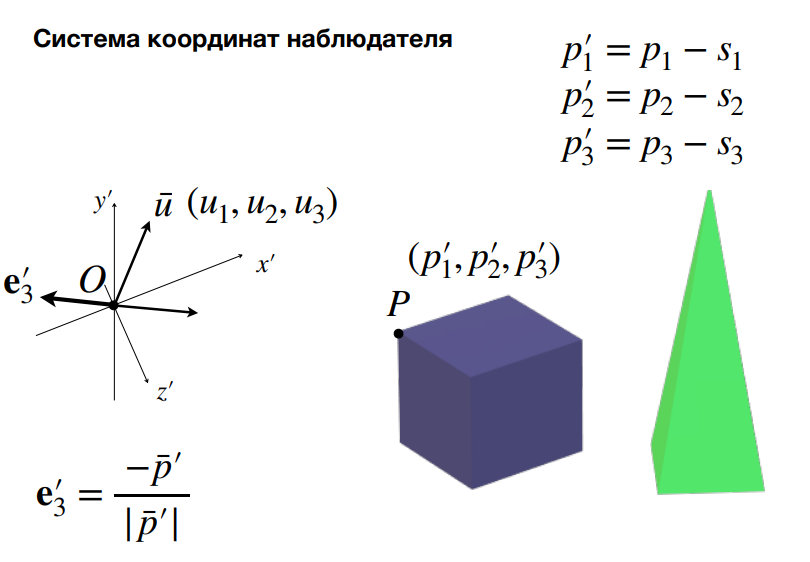
\includegraphics[width=0.70\linewidth]{Снимок экрана 2025-03-31 130326.png}
\end{figure}

Определить первый базисный вектор

Определить второй базисный вектор

Определить третий базисный вектор

\begin{figure} [H]
    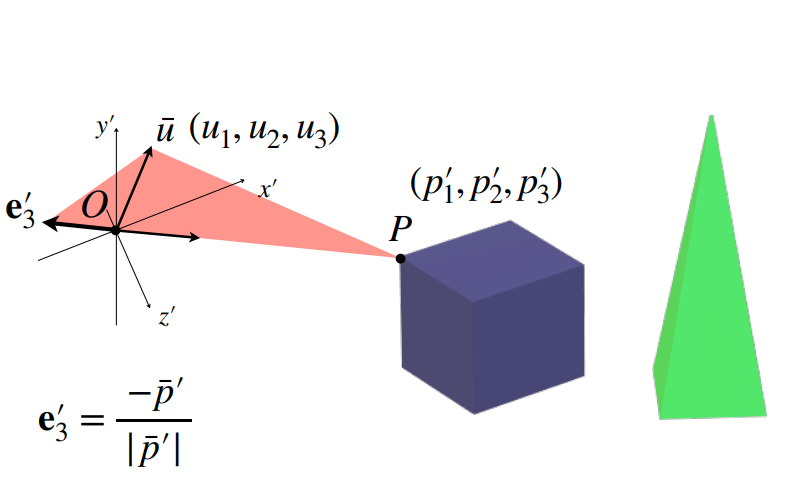
\includegraphics[width=0.70\linewidth]{Снимок экрана 2025-03-31 130527.png}
\end{figure}

После всех превращений нужно... 

LookAt - получет матрицу вращений. Преобразование системы переходы из  мировой системы координат
в ситсему координат наблюдателя

\begin{figure} [H]
    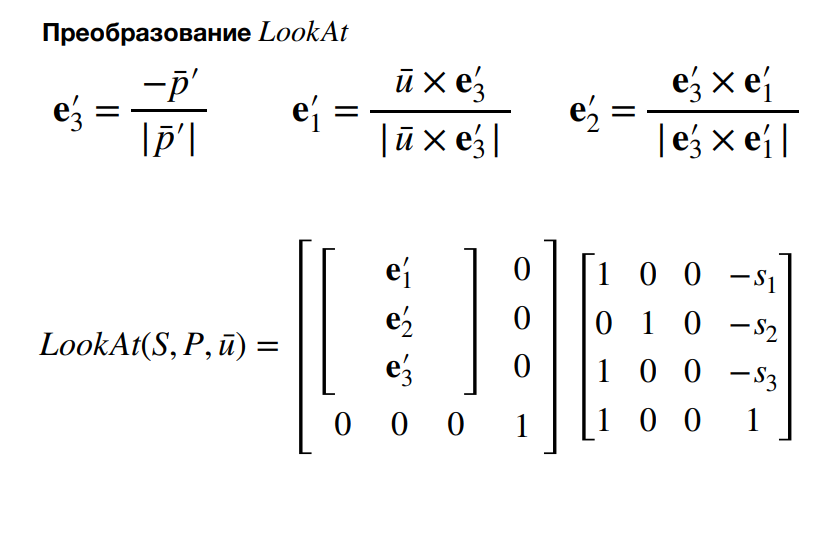
\includegraphics[width=0.70\linewidth]{Снимок экрана 2025-03-31 130706.png}
\end{figure}

Вверху на кортинке опечатка: лишняя единица и на глваной диагонали нехваетает единицы

\vspace{2mm}

$\begin{bmatrix}
    0 && 0 && 0 && -S_1 \\
    0 && 1 && 0 && -S_2 \\
    0 && 0 && 1 && -S_3 \\
    0 && 0 && 0 && 1 \\
\end{bmatrix}
$

\vspace{2mm}

Правильная матрица


Плоскость наблюдения (круг).

Окно наблюдения(квадрат) кадр

\begin{figure} [H]
    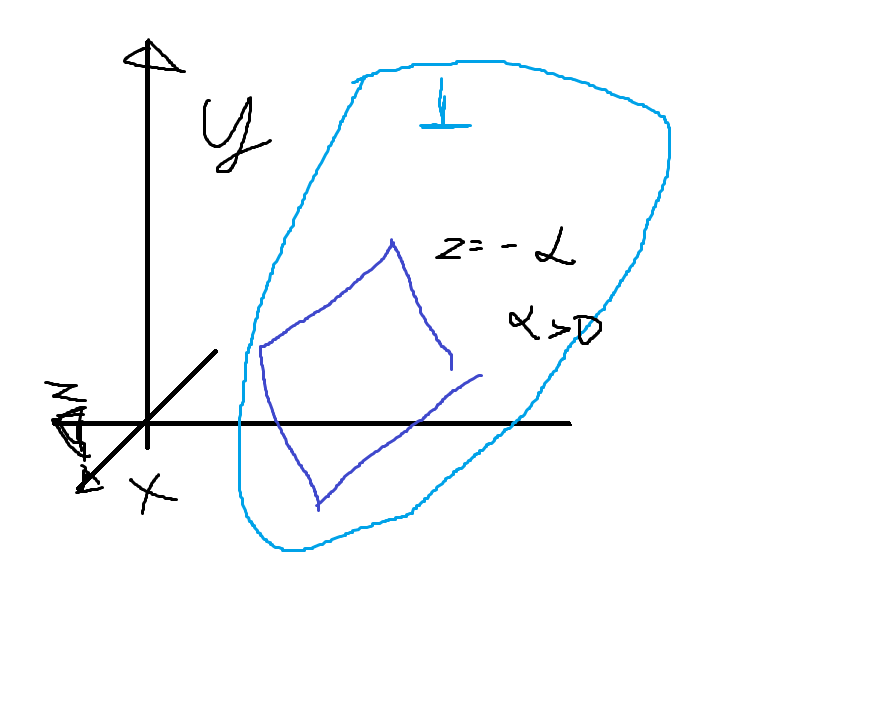
\includegraphics[width=0.70\linewidth]{набл.png}
\end{figure}

near - расстояние от наблюдателя до окна наблюдения

\section{Трехмерные преобазования}

\begin{figure} [H]
    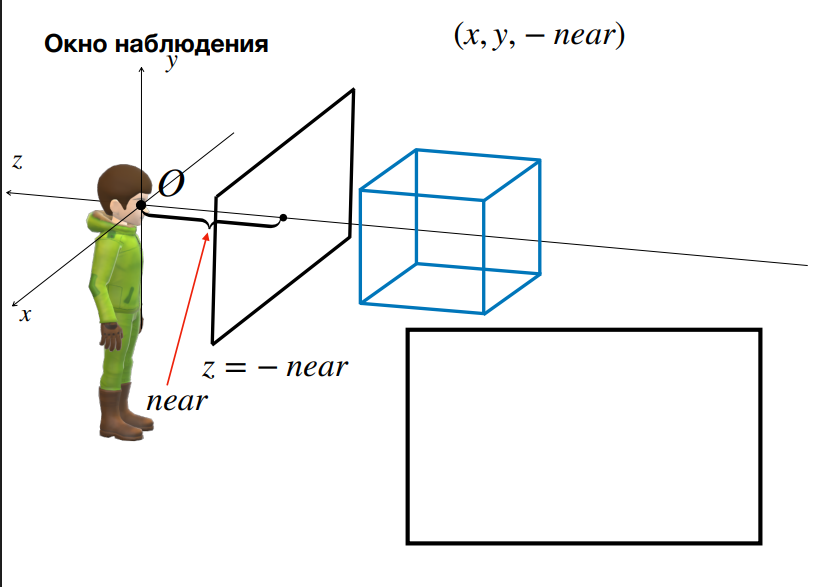
\includegraphics[width=0.70\linewidth]{Снимок экрана 2025-03-31 133559.png}
\end{figure}

Перспектива - это намернное искажения изображения с целью приданию глубины

\begin{figure} [H]
    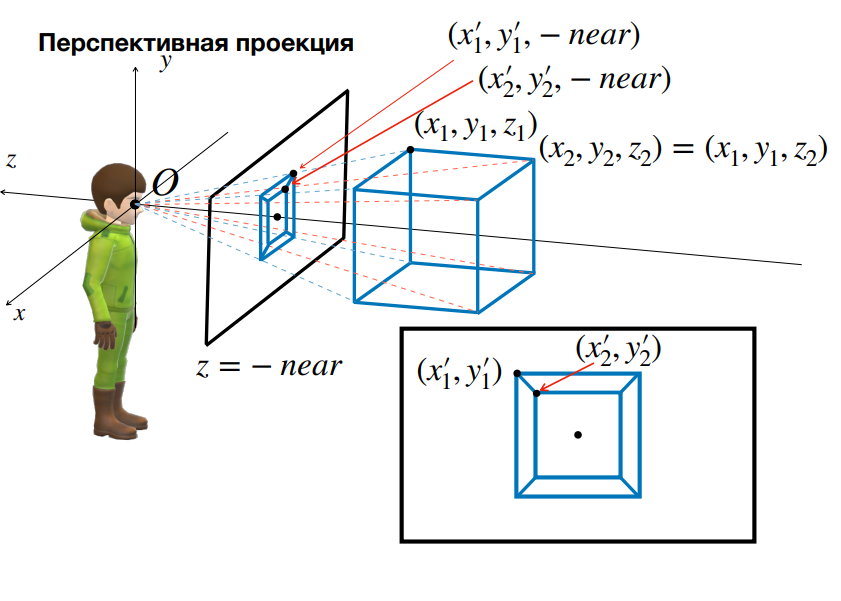
\includegraphics[width=0.70\linewidth]{Снимок экрана 2025-03-31 133646.png}
\end{figure}



\begin{figure} [H]
    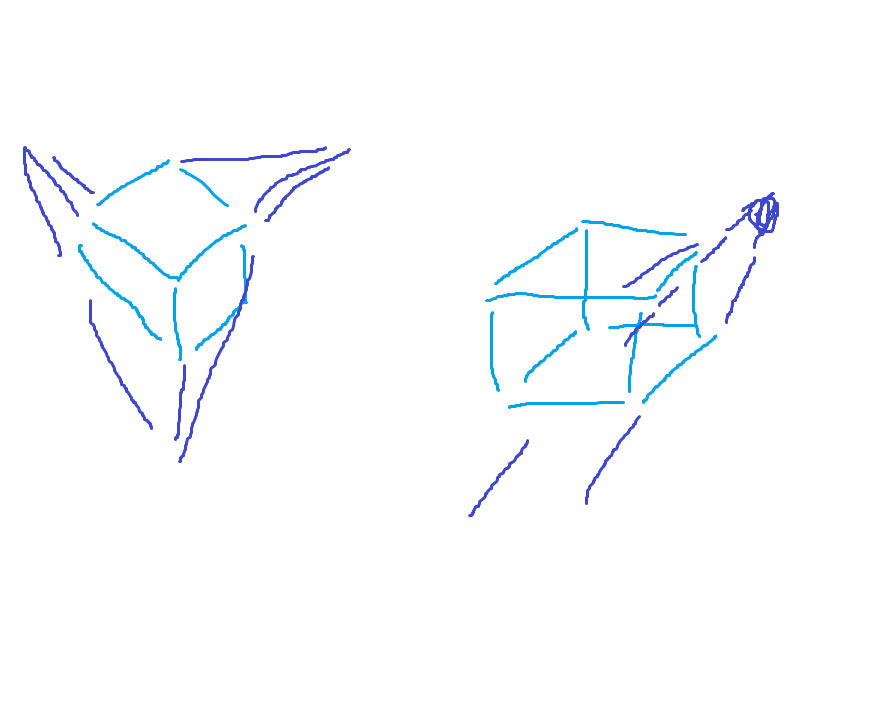
\includegraphics[width=0.70\linewidth]{куб.png}
\end{figure}

\subsection{Перспекитвное преобразование}






тут должно быть изображение с изображением того что на доске (смотреть в телефоне)


\begin{figure} [H]
    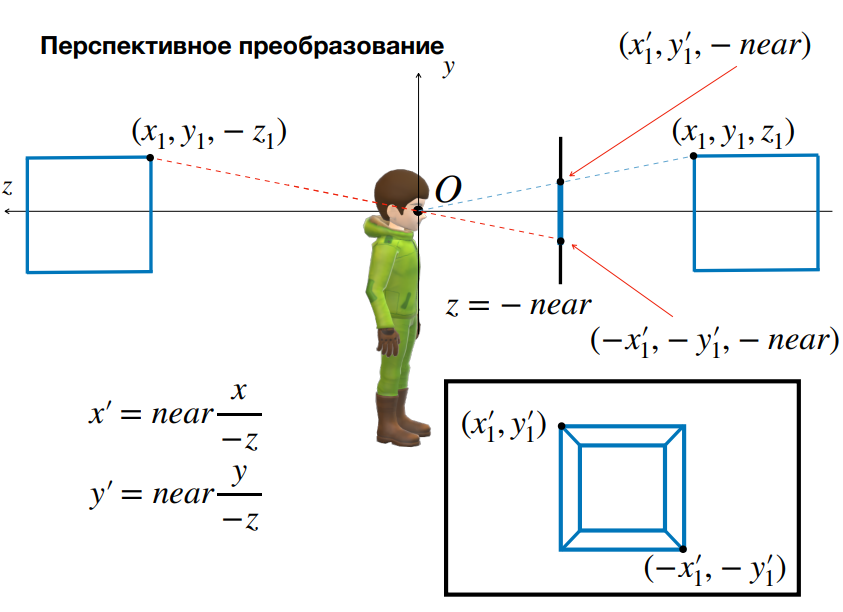
\includegraphics[width=0.70\linewidth]{Снимок экрана 2025-03-31 133818.png}
\end{figure}


\vspace{5cm}

\textbf{07.04.25}

\subsection{Отсечение невидмых частей сцены}


1) \textbf{Проволоченое} изрбражение - это объект заданный отрезками, 
здесь можно переспективное преобзразование применить,
или прямоугольная проекция.

2) Когда изображение задананно гранями оно называется \textbf{контурным}

Можно описать грани как: последовательность отрезков, 
получается мы описываем их как набор многоугольников.

3) \textbf{Полутонове} изображение у каждой грани есть атрибуты.

\begin{figure} [H]
    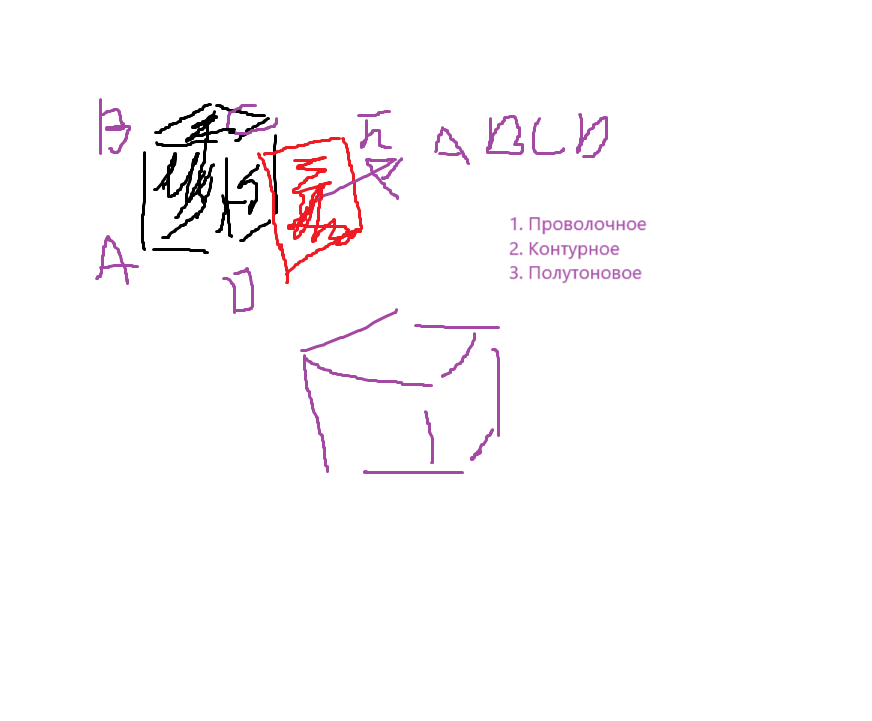
\includegraphics[width=0.70\linewidth]{prpov.png}
\end{figure}




\begin{figure} [H]
    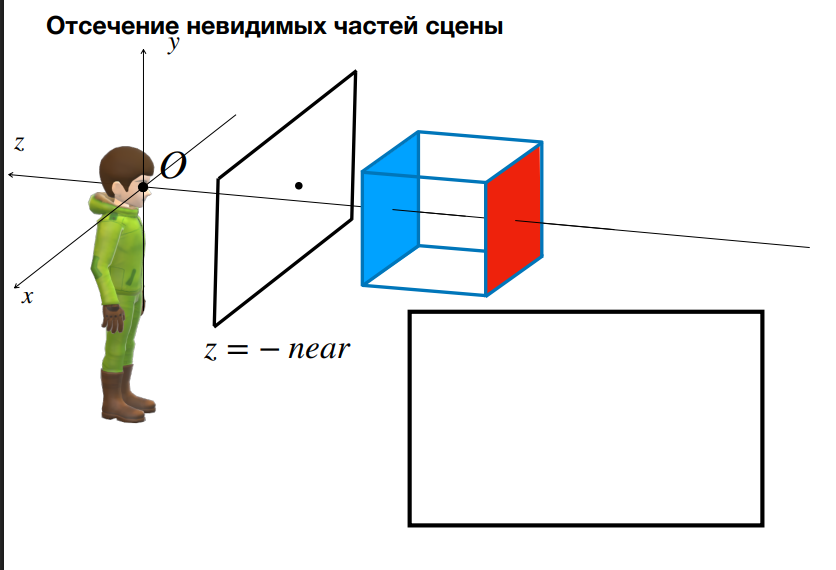
\includegraphics[width=0.70\linewidth]{Снимок экрана 2025-04-07 121652.png}
\end{figure}


\textbf{Отсечение}

\begin{figure} [H]
    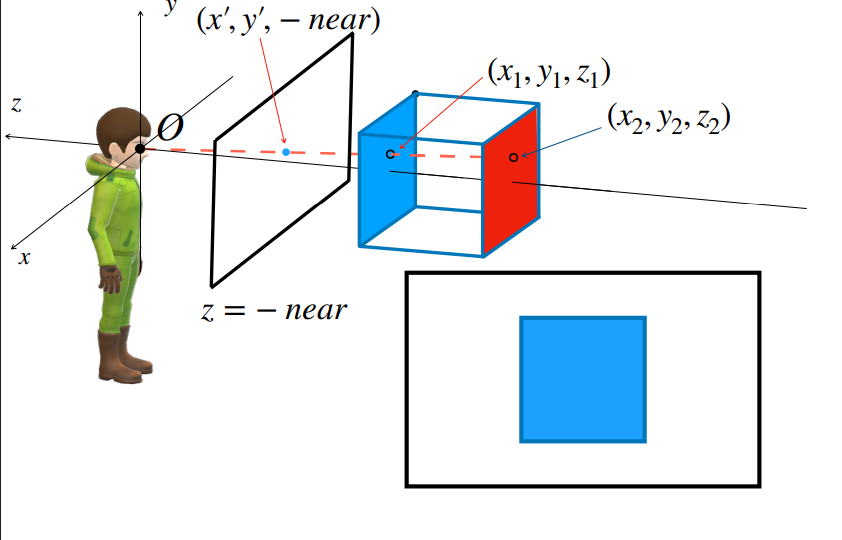
\includegraphics[width=0.70\linewidth]{Снимок экрана 2025-04-07 121741.png}
\end{figure}

\vspace{5cm}

\textbf{Простраснтво отсечения}

\begin{figure} [H]
    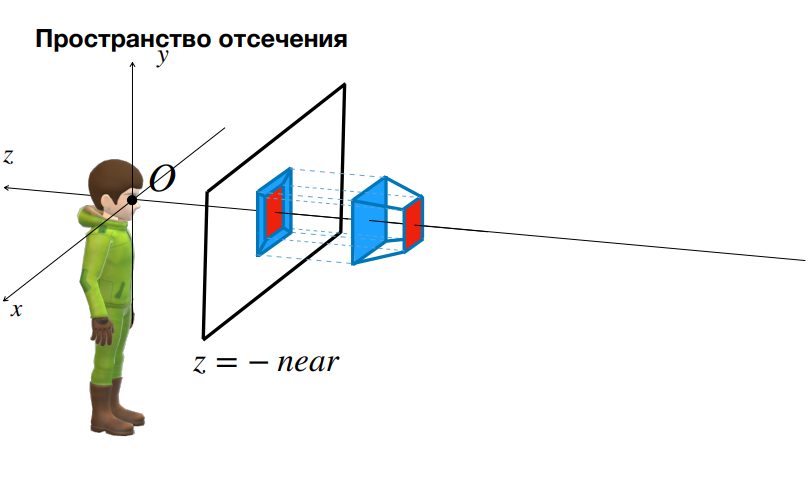
\includegraphics[width=0.70\linewidth]{Снимок экрана 2025-04-07 121816.png}
\end{figure}

\textbf{Пирамида видимости}

\begin{figure} [H]
    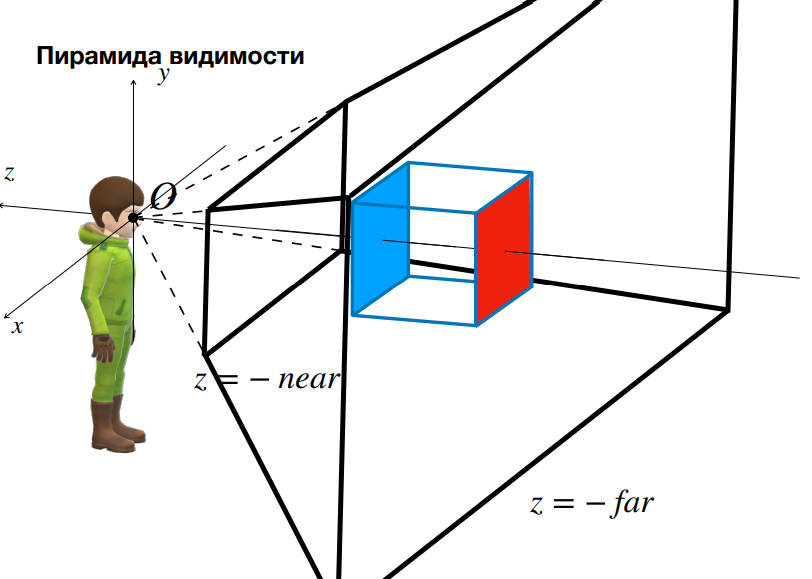
\includegraphics[width=0.70\linewidth]{Снимок экрана 2025-04-07 121910.png}
\end{figure}

\textbf{Пространство отсечения}

Система координат ростравнсвто отсечения - промежуточная система координат,
....... прямоугольная проекция.

Главный вопрос насколько мы далеко "отодвинули", "раздвинула"

В этом преобзравние оси x и z меняются местами. Система координат левая.

Будем говорить, что наблюдатель видит все что до far, за far его область
видимости пропадает.

far - расстояние

-far - координата

\textbf{FRUSTUM} - усеченная пирамида, по русски это называется пирамида видимости.
Она ограничина плоскостью горизонта, областью видимости наблюдателя.


\begin{figure} [H]
    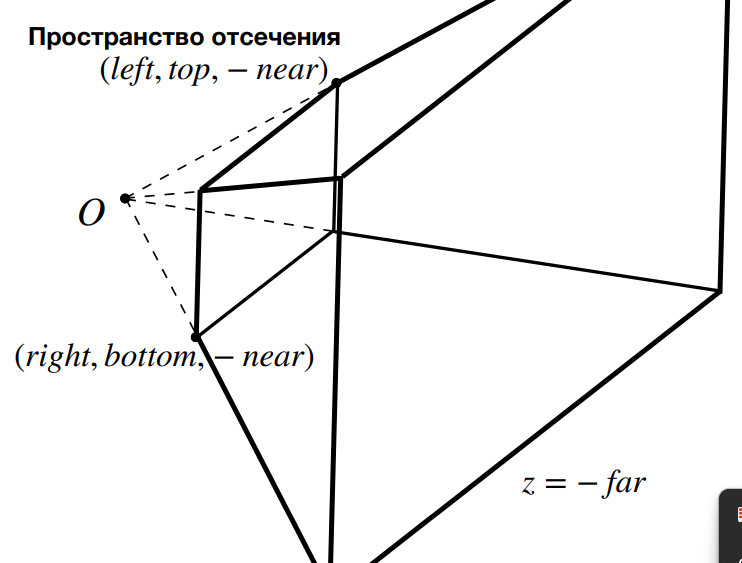
\includegraphics[width=0.70\linewidth]{Снимок экрана 2025-04-07 122337.png}
\end{figure}

Задаем окно наблюдения - оно ограниченно 

left,rirgt - x - параметры наблюдения, координаты

top, bottom - y - параметры наблюдения, координаты

Вся плоскость наблюдения ограниченна -near

near, far - расстояния

\begin{figure} [H]
    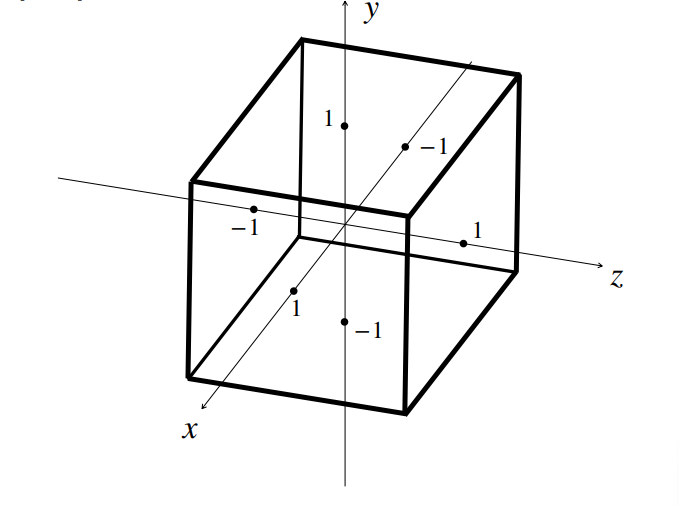
\includegraphics[width=0.70\linewidth]{Снимок экрана 2025-04-07 122342.png}
\end{figure}


\begin{figure} [H]
    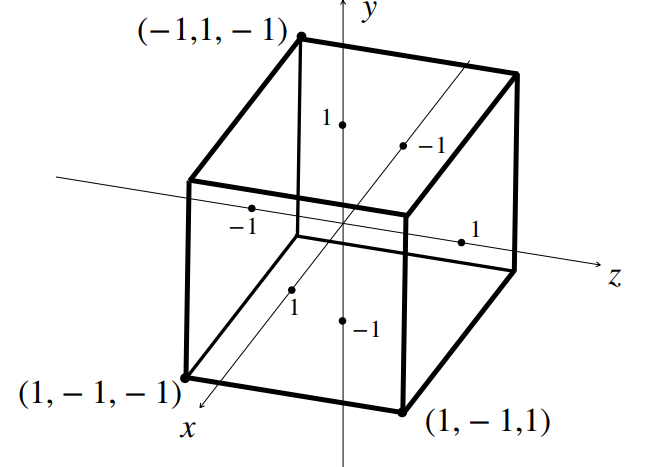
\includegraphics[width=0.70\linewidth]{Снимок экрана 2025-04-07 122403.png}
\end{figure}

\textbf{Переход в пространтсво отсечения}

Если взять окно наблюдения, то оно передет в одну из сторон куба, 
left,top,-near перейдет в (-1,1,-1), а
right,bottom,-near перейдет в (1,-1,-1),
z=-far перейдет в z=1

\vspace{1cm}

В начале нужно провести оперцию кодрирования

Это переспективное преобразование

$Vcx = left$     \hspace{2cm}  $Wcx = -1$

$Vcy = bottom$  \hspace{2cm}    $Wyx = -1$

$Vx = right-lefft$  \hspace{2cm} $Wy = 2$

$Vy = top-bottom$   \hspace{2cm} $Wy = 2$

$x" = \frac{x'right-lefft}{}$ это недописано

$y" = \frac{y'right-lefft}{}$ это недописано

А это переспективное проекция

$x"=\frac{\frac{nearx}{-z}-left}{right - left}*2-1$

$y"=\frac{\frac{neary}{-z}-bottom}{top - bottom}*2-1$






\begin{figure} [H]
    \includegraphics[width=0.70\linewidth]{Снимок экрана 2025-04-07 122537.png}
\end{figure}


\begin{figure} [H]
    \includegraphics[width=0.70\linewidth]{Снимок экрана 2025-04-07 122544.png}
\end{figure}

\begin{figure} [H]
    \includegraphics[width=0.70\linewidth]{Снимок экрана 2025-04-07 122640.png}
\end{figure}


А тперь преобразование
\vspace{5mm}

$x" =\frac{\frac{nearx+zleft}{-z}}{right - left}*2-1$

\vspace{5mm}

$x"=\frac{\frac{nearx+zlef}{right - left}}{-z}*2-1$

\vspace{5mm}

$x"=\frac{\frac{nearx+zlef}{right - left}}{-z}*2-1$

\begin{figure} [H]
    \includegraphics[width=0.70\linewidth]{Снимок экрана 2025-04-07 122649.png}
\end{figure}

\subsection{Матрица перспективного преобразования}

\begin{figure} [H]
    \includegraphics[width=0.70\linewidth]{Снимок экрана 2025-04-07 122839.png}
\end{figure}

$\alpha" = -z $

\begin{figure} [H]
    \includegraphics[width=0.70\linewidth]{Снимок экрана 2025-04-07 122852.png}
\end{figure}

\begin{figure} [H]
    \includegraphics[width=0.70\linewidth]{Снимок экрана 2025-04-07 122855.png}
\end{figure}

\begin{figure} [H]
    \includegraphics[width=0.70\linewidth]{Снимок экрана 2025-04-07 122904.png}
\end{figure}

\begin{figure} [H]
    \includegraphics[width=0.70\linewidth]{Снимок экрана 2025-04-07 123233.png}
\end{figure}

\begin{figure} [H]
    \includegraphics[width=0.70\linewidth]{Снимок экрана 2025-04-07 123325.png}
\end{figure}

\begin{figure} [H]
    \includegraphics[width=0.70\linewidth]{Снимок экрана 2025-04-07 123353.png}
\end{figure}

\begin{figure} [H]
    \includegraphics[width=0.70\linewidth]{Снимок экрана 2025-04-07 123428.png}
\end{figure}


$\frac{a_{34}}{-far} - \frac{a_{34}}{-near} = -2$




\begin{figure} [H]
    \includegraphics[width=0.70\linewidth]{Снимок экрана 2025-04-07 123451.png}
\end{figure}

\begin{figure} [H]
    \includegraphics[width=0.70\linewidth]{Снимок экрана 2025-04-07 123520.png}
\end{figure}

Эта матрица зависит от этих параметров

тут можно еще можно дополнить (произошел спидран лекции), вот час побудет подробнее




\vspace{1cm}


\textbf{14.04.25}


Модельная система коордниат(МСК) $\implies^{model veiew}$ Мировая система координат $\implies^{LookAt}$ СКН 
$\implies ^{FRUSTUM}$ СКПО

far y field f view Oy

aspect aspect ratio

near

far


Частный случай:

left right

bottop top

near far

\begin{figure} [H]
    \includegraphics[width=0.70\linewidth]{прям.png}
\end{figure}

\begin{figure} [H]
    \includegraphics[width=0.70\linewidth]{Снимок экрана 2025-04-14 125319.png}
\end{figure}

Матрица частного слуя преобразоавания



$\begin{bmatrix}
    \chi \\ 
    \gamma \\
    \zeta \\
    \alpha \\
\end{bmatrix}$
=
$\begin{bmatrix}
    \frac{1}{aspect}ctg\frac{fovy}{2} & 0 & 0 & 0 \\
    0 & ctg\frac{fovy}{2} & 0 & 0 \\
    0 & 0 & -\frac{far+near}{far-near} & \frac{-2far*near}{far-ner} \\
    0 & 0 & -1 & 0 \\
\end{bmatrix}$
=
$\begin{bmatrix}
    x\\
    y\\
    z\\
    1\\
\end{bmatrix}$

Perspective(fovy,aspect,near,far)

\vspace{5cm}

\textbf{Прямоугольная проекция}


\begin{figure} [H]
    \includegraphics[width=0.70\linewidth]{Снимок экрана 2025-04-14 125703.png}
\end{figure}


$x'=\frac{x-Vcx}{Vx}Wx+Wcx$ \vspace{1cm} Vx = right-left

$y'=\frac{y-Vcy}{Vy}Wy+Wcy$ \vspace{1cm} Vy = top-bottom

$z'= Wcx- \frac{z-Vcz}{Vz}Wz$   \vspace{1cm} Vz = far-near

(-1,-1,-1)
\vspace{1mm}
Wcx=Wcy+Wcz
\vspace{1mm}

$x'=\frac{x-left}{righht-left}2-1$ \vspace{1cm} = $\frac{2x}{right-left}+\frac{-2left-right+left}{right-left}$

$y'=\frac{y-Vcy}{top-bottom}2-1y$ \vspace{1cm} = $\frac{2y}{top-botton}+\frac{-2bottom-top+bottom}{top-bottom}$

$z'= -1 - \frac{z+near}{far-near}2$   \vspace{1cm} = $\frac-{2z}{far-near}+\frac{-2near-far+near}{far-near}$


\vspace{5cm}
Матрица преобразование Ortho. В основном используется в OpenGL

\begin{figure} [H]
    \includegraphics[width=0.70\linewidth]{Снимок экрана 2025-04-14 131345.png}
\end{figure}




\section{Организация движения в трехмерном пространтсве}

\begin{figure} [H]
    \includegraphics[width=0.70\linewidth]{Снимок экрана 2025-04-14 133843.png}
\end{figure}



Чтобы применить преобразование LookAt нужно:

1. В которую переходит глаз наблюдателя

2. Точка в которую смотрит наблюдатель

3. Вектор направление вверх

LookAt(S,P,$\bar{u}$)


LookAt((0,0,-1),(0,0,-2),(0,1,0))

LookAt((0,0,1),(0,0,0),(0,1,0))

и т.д 

Подобное происходит и напрвалением вверх/вниз

LookAt((0,1,0),(0,1,-1),(0,1,0))

и т.д


\vspace{1cm}

\textbf{21.04.25}


Для двежиения достаточно умнажать обшую матрицу на матрицу Tr, P и т.д
$(0(T_r*Rot*T_r*L*M)*P)$ это преобразование LookAt.



\textbf{Совмещенное преобразование}


\begin{figure} [H]
    \includegraphics[width=0.70\linewidth]{Снимок экрана 2025-04-21 122739.png}
\end{figure}



$\begin{bmatrix}
    1 & 0 & 0 & T_x \\
    0 & 1 & 0 & T_y \\
    0 & 0 & 1 & T_z \\
    0 & 0 & 0 & T \\ 
\end{bmatrix} $

$P=M^{-1}MP$



\section{Алгоритм Коэна-Сазерленда}

\textbf{Алгоритм обязятельно знать, без него не сдать экзамен!}


\begin{figure} [H]
    \includegraphics[width=0.70\linewidth]{отс.png}
\end{figure}



\vspace{5mm}

Пропус

\vspace{5mm}

\textbf{05.05.25}

\section{Растеризация}


\begin{figure} [H]
    \includegraphics[width=0.70\linewidth]{Снимок экрана 2025-05-05 121851.png}
\end{figure}


\begin{figure} [H]
    \includegraphics[width=0.70\linewidth]{Снимок экрана 2025-05-05 122011.png}
\end{figure}



Для каждого из остальных ребер формируем тройку, где первый элемент равен $X_1$, 
второй (это не точно, не расслышала про второй элемент)$Z_1$,третий $Y_1$.


\begin{figure} [H]
    \includegraphics[width=0.70\linewidth]{Снимок экрана 2025-05-05 122144.png}
\end{figure}


$x_1 0$

$(r_1,g_1,b_1)$

$x_2-x_1+1$

\vspace{1mm}

$x_2$

$(r_2,g_2,b_2)$

По сути это цвтеовой шаг. $x_2-x_1+1$ - отрезок


\begin{figure} [H]
    \includegraphics[width=0.70\linewidth]{Снимок экрана 2025-05-05 123436.png}
\end{figure}


Если мы предполагем, что у нас есть z, то она будет, такаже изменяться как и x и y.

\begin{figure} [H]
    \includegraphics[width=0.70\linewidth]{Снимок экрана 2025-05-05 123643.png}
\end{figure}


\subsection{Алгоритм использующий Z-буфер}

\begin{figure} [H]
    \includegraphics[width=0.70\linewidth]{Снимок экрана 2025-05-05 125223.png}
\end{figure}


\begin{figure} [H]
    \includegraphics[width=0.70\linewidth]{Снимок экрана 2025-05-05 124350.png}
\end{figure}


\textbf{Z-буфер} это двумерный массив, 
в котором столько элементов сколько стоблцов и сколько строк растра.


\section{Графический конвейр в OpenGL}


\textbf{Построение трехмерного прообраза}

\textbf{modelView} - Модельное преобзравние (переход в мировую систему координат).

\textbf{cameraView} - Переход в систему координат наблюдателя.

\textbf{OpenGL} - это НЕ библиотека, это прежде всего спецификация, которая должна
удевлитворяеть графическая карта, которую мы покупаем.

Спецификация - (техническое задание) предполагает

\end{document}